% Results
% 1: correct
% 2: incorrect NL
% 3: incorrect SL
% 4: bad question
% 5: confused
% date
% Avg. minutes: 18.528333333333332
% Bad: 0
% 33 [4. 3. 3.]
% Krippendorffs Agreement: 0.14715969989281902
% Observed Agreement: 0.7878787878787878
% {'1': 0, '3': 1, '4': 2, '2': 3}
% Percent selected: [0.85454545 0.10909091 0.00909091 0.02727273]

% Relation
% Avg. minutes: 24.816666666666666
% Bad: 0
% 100 [4. 3. 3. 4. 3. 2. 3. 3. 3. 4.]
% Krippendorffs Agreement: 0.08618796662274913
% Observed Agreement: 0.6833333333333332
% {'2': 0, '1': 1, '2,4': 2, '4,5': 3, '3': 4, '5': 5, '4': 6}
% Percent selected: [0.05625  0.815625 0.003125 0.003125 0.040625 0.025    0.05625 ]

% mwp
% Avg. minutes: 19.28709677419355
% Bad: 0
% 100 [3. 3. 2. 4. 3. 3. 3. 3. 4. 3.]
% Krippendorffs Agreement: 0.13477933801404238
% Observed Agreement: 0.7899999999999998
% {'3,4': 0, '2': 1, '1': 2, '2,3': 3, '3': 4, '5': 5, '2,3,4': 6, '4': 7}
% Percent selected: [0.00322581 0.02580645 0.86451613 0.01290323 0.02903226 0.02580645
%  0.00322581 0.03548387]

% sports
% Avg. minutes: 14.52962962962963
% Bad: 0
% 33 [3. 3. 3.]
% Krippendorffs Agreement: -0.025104602510461902
% Observed Agreement: 0.8989898989898989
% {'1': 0, '2,3': 1, '5': 2, '2': 3}
% Percent selected: [0.94949495 0.02020202 0.01010101 0.02020202]

% strategyqa
% Avg. minutes: 26.033333333333335
% Bad: 0
% 33 [3. 3. 3.]
% Krippendorffs Agreement: 0.013790532985464109
% Observed Agreement: 0.45454545454545453
% {'2': 0, '1': 1, '2,3': 2, '3': 3, '5': 4, '4': 5}
% Percent selected: [0.21212121 0.62626263 0.02020202 0.12121212 0.01010101 0.01010101]

 % We know that the generated code is a faithful explanation for the final answer that we produce, but we cannot guarantee that the explanation actually corresponds to the question. 
In our main experiments, we use final answer accuracy to measure performance, but this metric does not necessarily correspond to the validity of the reasoning chain. Technically, a model can sometimes accidentally arrive at the correct answer with a wrong reasoning chain.
% In our experiments, we use answer accuracy as the evaluation metric, but a model can also accidentally produce a correct answer when the reasoning chain is not reasonable, resulting in false positives.
Precisely, we want to know: \textbf{when the answer is correct, how often is the reasoning chain truly correct?} Since there is no ground truth to compare the reasoning chains with, we conduct a human evaluation study on Prolific: given a generated reasoning chain from the Translation stage which results in a correct answer, a crowd-worker selects whether it is \textit{A) completely correct}, or, if incorrect, specify why with \textit{B) incorrect NL} and/or \textit{C) incorrect SL}. Alternatively, they can select \textit{D) flawed question} and \textit{E) I am confused}. 

\begin{figure}
    \centering
    % https://drive.google.com/file/d/1L-RJFSLhTjXjD0lR0hK-hA5SO8bV6euc/view?usp=sharing
    \includegraphics[width=0.99\linewidth]{fables/human_eval-3.pdf}
    \caption{Human evaluation results of reasoning chain correctness. Each column represents the percent of different answer choices selected by human evaluators in each domain/dataset.}
    \label{fig:human_eval}
\end{figure}

\begin{table*}[h]
    \centering
    \vskip 0.15in
    \small
    \begin{tabular}{lrrrrr|r}
         \toprule
         Domain &  Correct & Incorrect NL & Incorrect SL & Flawed Question & Confused & Agreement\\
         \midrule
         MWP & 92.0 & 3.0 & 2.0 & 2.0 & 1.0 & 0.790\\
         Planning & 94.0 & 3.9 & 2.1 & 0.0 & 0.0 & 0.947\\         
         StrategyQA & 66.7 & 30.3 & 3.0 & 0.0 & 0.0 & 0.455\\         
         Date & 87.9 & 6.1 & 6.1 & 0.0 & 0.0 & 0.788\\
         Sports & 100.0 & 0.0 & 0.0 & 0.0 & 0.0 & 0.899\\         
         Relation & 88.0 & 6.0 & 0.0 & 5.0 & 1.0 & 0.683\\
         \bottomrule
    \end{tabular}
\caption{Numerical results for human evaluation of reasoning chain correctness, accompanying Figure~\ref{fig:human_eval}. Each row represents the percent (0-100) of different answer choices selected by human evaluators in each domain/dataset, as well as the inter-annotator agreement.}
    \label{tab:human_eval}
\end{table*}


We hire crowd workers on Prolific to evaluate the correctness of model-generated reasoning chains that result in a correct answer. We sample 100 reasoning chains for each domain generated by \texttt{code-davinci-002} with the greedy decoding strategy, where each set of 100 contains an equal number of samples from all datasets within the domain. We further require annotators to have experience coding in the programming language of the dataset they annotate (Python for MWP/CLUTRR/Sports/Date, and Scala for StrategyQA, as Datalog was not an option in Prolific). We have a single survey for each domain, with the exception of Multi-hop QA (in this case, we have separate surveys for StrategyQA, Date, and Sports, given the different nature of each dataset). Additionally, there was no way to ensure annotators knew PPDL on Prolific. In order to ensure high-quality annotations for SayCan, the authors annotate this dataset themselves. 

\begin{figure}
    \centering
    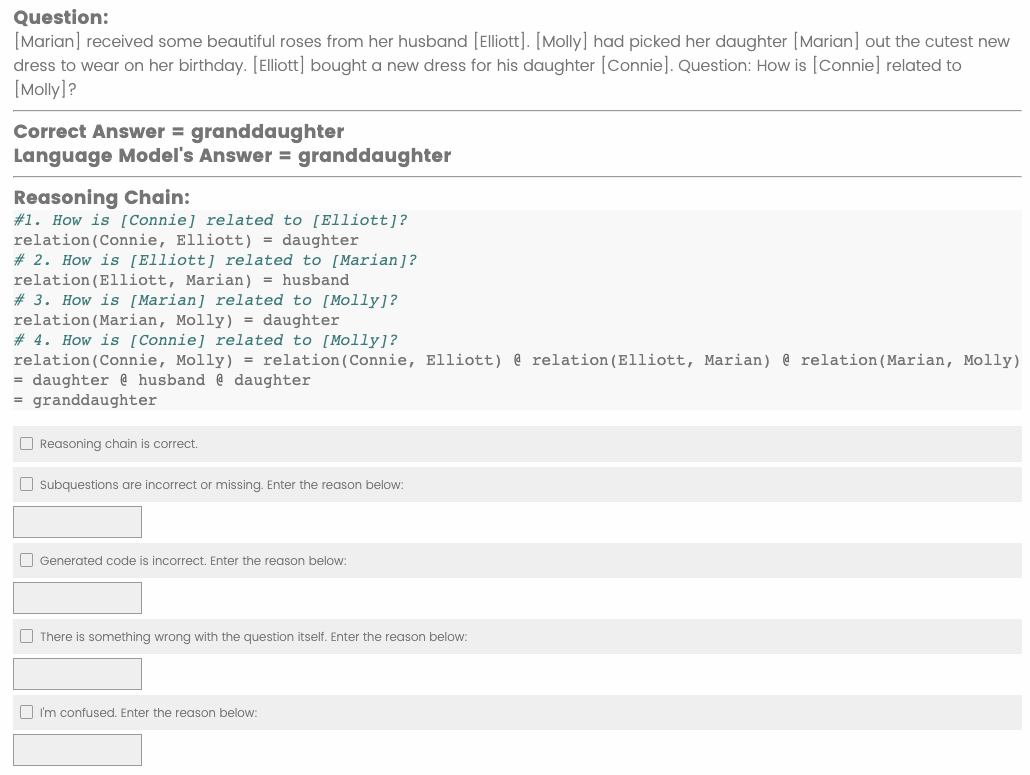
\includegraphics[width=\linewidth]{img/human_study_interface.png}
    \caption{Example of our annotation interface for the CLUTRR survey}
    \label{fig:interface}
\end{figure}

\paragraph{Annotation Process} Each of the 100 questions for each domain is annotated by at least three annotators. Each annotator is given 10 questions to annotate. A screenshot of our survey interface is shown in Figure~\ref{fig:interface}. At the start of the survey, annotators are given examples of a correct reasoning chain, a reasoning chain with incorrect NL, and a reasoning chain with incorrect SL. The examples match the domain of reasoning chains in each survey. As an attention and understanding check, we ask annotators to label an example they had just seen. If the annotator fails this question, they are sent to the end of the survey and their responses are filtered out. We also manually filter out all spammers (annotators who answer with the same response repeatedly or complete the survey in under 3 minutes). After the surveys are complete, we compute annotator agreement and then take the majority label for each reasoning chain as the final label in our analysis.
Our annotator population consists of 100 annotators with an average age of 25 years and an average income of 40k per year. 87.9\% of the annotators are males and 56\% have a four year college degree.
Annotators are compensated at \$16/hr, and average 2 minutes per question. Our full study cost \$280. Sample instructions for the CLUTRR survey can be found in the Supplementary Materials.

The results of our study are shown in Figure~\ref{fig:human_eval} and Table~\ref{tab:human_eval}. For most domains, we see that annotators often find the reasoning chain fully correct -- Sports, SayCan, and MWP have a 90\%+ correctness rate. To gain more insight into when the reasoning chain can be "incorrect", we perform an in-depth analysis of user annotations for the three worst-performing datasets -- StrategyQA (66.7\% correctness), Date (87.9\% correctness), and CLUTRR (88.0\% correctness). From our inspection, we find that annotators mistakenly mark a correct reasoning chain as incorrect at different rates based on the task (8.3\% of the time for StrategyQA, 41.7\% for Date Understanding, and 100\% for CLUTRR). We find annotators are inaccurate for Date because they incorrectly believe the generated code misuses a Python library (\texttt{relativedelta}), or they complain that there is a better way to answer the question. For CLUTRR, annotators mark chains as incorrect due to perceived ambiguity in the CLUTRR dataset. For example, the grandmother of one's child may not necessarily be their parent, but also a parent-in-law.

As for the remaining truly incorrect reasoning chains, we find the LM can sometimes add unnecessary steps or arrive at the correct answer by chance. The latter is especially an issue in StrategyQA - given that all questions have a True/False answer, it is common for an incorrect reasoning chain to result in a correct answer. For example, the LM correctly answers the question "Was Karachi a part of Alexander the Great's success?" as "True." However, the reasoning chain contains the flawed subquestion "Which countries are in Pakistan? Pakistan includes Pakistan, Afghanistan, and India." Though the final answer is correct and faithful to the LM generation, the reasoning chain contains wrong knowledge.


Overall, Faithful CoT does generate valid reasoning chains for the vast majority of the time when the answer is correct. However, we still see exceptions where the model arrives at the right answer via an incorrect reasoning chain. Though this happens rarely, our human study raises concerns about the trust people place in LMs. CoT-style methods that result in a correct answer do not guarantee that the reasoning chain is valid and plausible. To our knowledge, we are the first to conduct a systematic human study on the validity of reasoning chains, and we hope to see future work further investigate and improve on the flaws that our study brings to light. 